\documentclass[12pt, a4paper]{article}

% ── Page geometry ──────────────────────────────────────────────────────────────
\usepackage[a4paper, top=2.5cm, bottom=2.5cm, left=2.8cm, right=2.8cm,
            headheight=15pt]{geometry}

% ── Font & encoding ────────────────────────────────────────────────────────────
\usepackage[T1]{fontenc}
\usepackage[utf8]{inputenc}
\usepackage{palatino}
\usepackage{mathpazo}
\usepackage{microtype}

% ── Maths ─────────────────────────────────────────────────────────────────────
\usepackage{amsmath, amssymb, amsthm, mathtools}
\usepackage{cancel}

% ── Graphics & colour ─────────────────────────────────────────────────────────
\usepackage{xcolor}
\usepackage{tikz}
\usetikzlibrary{arrows.meta, positioning, calc, shapes.geometric,
                decorations.pathreplacing, backgrounds, fit, patterns}
\usepackage{pgfplots}
\pgfplotsset{compat=1.15}

% ── Tables ────────────────────────────────────────────────────────────────────
\usepackage{booktabs, array, colortbl, multirow, tabularx}
\renewcommand{\arraystretch}{1.4}

% ── Lists ─────────────────────────────────────────────────────────────────────
\usepackage{enumitem}
\setlist[itemize]{leftmargin=1.8em, itemsep=3pt, topsep=4pt}
\setlist[enumerate]{leftmargin=1.8em, itemsep=3pt, topsep=4pt}

% ── Boxes ─────────────────────────────────────────────────────────────────────
\usepackage[most]{tcolorbox}
\tcbuselibrary{skins, breakable, theorems}

% ── Headers & footers ─────────────────────────────────────────────────────────
\usepackage{fancyhdr}
\usepackage{lastpage}

% ── Hyperlinks ────────────────────────────────────────────────────────────────
\usepackage[colorlinks=true, linkcolor=royalblue, urlcolor=royalblue,
            citecolor=royalblue, bookmarks=true]{hyperref}
\usepackage{tocloft}

% ── Miscellaneous ─────────────────────────────────────────────────────────────
\usepackage{parskip}
\setlength{\parskip}{6pt}
\setlength{\parindent}{0pt}
\usepackage{float}
\usepackage{caption}

% ═══════════════════════════════════════════════════════════════════════════════
%  COLOUR PALETTE  (deep navy / gold / teal)
% ═══════════════════════════════════════════════════════════════════════════════
\definecolor{royalblue}{RGB}{25, 55, 130}
\definecolor{navylight}{RGB}{235, 239, 252}
\definecolor{navyborder}{RGB}{100, 130, 200}
\definecolor{gold}{RGB}{185, 135, 15}
\definecolor{lightgold}{RGB}{254, 248, 225}
\definecolor{teal}{RGB}{15, 115, 105}
\definecolor{lightteal}{RGB}{225, 248, 244}
\definecolor{tealborder}{RGB}{15, 115, 105}
\definecolor{crimson}{RGB}{155, 25, 35}
\definecolor{lightcrimson}{RGB}{255, 235, 235}
\definecolor{purple}{RGB}{88, 35, 140}
\definecolor{lightpurple}{RGB}{245, 238, 255}
\definecolor{charcoal}{RGB}{42, 42, 42}
\definecolor{slategray}{RGB}{80, 90, 105}
\definecolor{tabhead}{RGB}{25, 55, 130}
\definecolor{tabeven}{RGB}{235, 240, 252}
\definecolor{solgreen}{RGB}{12, 100, 55}
\definecolor{lightsol}{RGB}{228, 252, 238}

% ═══════════════════════════════════════════════════════════════════════════════
%  TCOLORBOX ENVIRONMENTS
% ═══════════════════════════════════════════════════════════════════════════════

\newtcolorbox{defbox}[1]{
  breakable, enhanced,
  colback=navylight, colframe=royalblue, coltitle=white,
  fonttitle=\bfseries\sffamily, title={Definition: #1},
  arc=4pt, boxrule=1pt, left=8pt, right=8pt, top=6pt, bottom=6pt,
  attach boxed title to top left={yshift=-2mm, xshift=6mm},
  boxed title style={colback=royalblue, arc=3pt, boxrule=0pt}
}

\newtcolorbox{thmbox}[1]{
  breakable, enhanced,
  colback=lightteal, colframe=teal, coltitle=white,
  fonttitle=\bfseries\sffamily, title={Theorem: #1},
  arc=4pt, boxrule=1pt, left=8pt, right=8pt, top=6pt, bottom=6pt,
  attach boxed title to top left={yshift=-2mm, xshift=6mm},
  boxed title style={colback=teal, arc=3pt, boxrule=0pt}
}

\newtcolorbox{propbox}[1]{
  breakable, enhanced,
  colback=lightteal, colframe=teal, coltitle=white,
  fonttitle=\bfseries\sffamily, title={Proposition: #1},
  arc=4pt, boxrule=1pt, left=8pt, right=8pt, top=6pt, bottom=6pt,
  attach boxed title to top left={yshift=-2mm, xshift=6mm},
  boxed title style={colback=teal, arc=3pt, boxrule=0pt}
}

\newtcolorbox{keybox}[1]{
  breakable, enhanced,
  colback=lightgold, colframe=gold, coltitle=charcoal,
  fonttitle=\bfseries\sffamily, title={#1},
  arc=4pt, boxrule=1pt, left=8pt, right=8pt, top=6pt, bottom=6pt,
  attach boxed title to top left={yshift=-2mm, xshift=6mm},
  boxed title style={colback=gold, arc=3pt, boxrule=0pt, coltitle=white}
}

\newtcolorbox{exbox}[1]{
  breakable, enhanced,
  colback=lightpurple, colframe=purple, coltitle=white,
  fonttitle=\bfseries\sffamily, title={Worked Example: #1},
  arc=4pt, boxrule=1pt, left=8pt, right=8pt, top=6pt, bottom=6pt,
  attach boxed title to top left={yshift=-2mm, xshift=6mm},
  boxed title style={colback=purple, arc=3pt, boxrule=0pt}
}

\newtcolorbox{warnbox}[1]{
  breakable, enhanced,
  colback=lightcrimson, colframe=crimson, coltitle=white,
  fonttitle=\bfseries\sffamily, title={#1},
  arc=4pt, boxrule=1pt, left=8pt, right=8pt, top=6pt, bottom=6pt,
  attach boxed title to top left={yshift=-2mm, xshift=6mm},
  boxed title style={colback=crimson, arc=3pt, boxrule=0pt}
}

\newtcolorbox{solbox}{
  breakable, enhanced,
  colback=lightsol, colframe=solgreen, coltitle=white,
  fonttitle=\bfseries\sffamily, title={Solution},
  arc=4pt, boxrule=1pt, left=8pt, right=8pt, top=6pt, bottom=6pt,
  attach boxed title to top left={yshift=-2mm, xshift=6mm},
  boxed title style={colback=solgreen, arc=3pt, boxrule=0pt}
}

% ── Theorem-style environments ─────────────────────────────────────────────────
\theoremstyle{definition}
\newtheorem{remark}{Remark}[section]
\newtheorem{corollary}{Corollary}[section]

% ═══════════════════════════════════════════════════════════════════════════════
%  MATHS MACROS
% ═══════════════════════════════════════════════════════════════════════════════
\newcommand{\R}{\mathbb{R}}
\newcommand{\N}{\mathbb{N}}
\newcommand{\Z}{\mathbb{Z}}
\newcommand{\Q}{\mathbb{Q}}
\newcommand{\C}{\mathbb{C}}
\newcommand{\Rn}{\mathbb{R}^n}
\newcommand{\Rm}{\mathbb{R}^m}
\newcommand{\powerset}{\mathcal{P}}
\newcommand{\st}{\;\text{s.t.}\;}
\newcommand{\xto}[1]{\xrightarrow{#1}}
\newcommand{\inv}{^{-1}}
\DeclareMathOperator{\dom}{dom}
\DeclareMathOperator{\ran}{ran}
\DeclareMathOperator{\img}{img}

% ── Table helpers ──────────────────────────────────────────────────────────────
\newcommand{\thead}[1]{\cellcolor{tabhead}\color{white}\textbf{#1}}

% ═══════════════════════════════════════════════════════════════════════════════
%  PAGE STYLE
% ═══════════════════════════════════════════════════════════════════════════════
\pagestyle{fancy}
\fancyhf{}
\fancyhead[L]{\textcolor{royalblue}{\textbf{ECON 320}} \textcolor{slategray}{--- Sets \& Functions}}
\fancyhead[R]{\textcolor{slategray}{\small School of Economics}}
\fancyfoot[C]{\textcolor{slategray}{\small Page \thepage\ of \pageref{LastPage}}}
\renewcommand{\headrulewidth}{1.2pt}
\renewcommand{\headrule}{%
  \hbox to\headwidth{\color{royalblue}\leaders\hrule height\headrulewidth\hfill}}
\renewcommand{\footrulewidth}{0.4pt}

% ── TOC styling ───────────────────────────────────────────────────────────────
\renewcommand{\cftsecfont}{\bfseries\color{royalblue}}
\renewcommand{\cftsecpagefont}{\bfseries\color{royalblue}}
\renewcommand{\cftsubsecfont}{\color{charcoal}}
\setlength{\cftbeforesecskip}{4pt}

% ═══════════════════════════════════════════════════════════════════════════════
\begin{document}
% ═══════════════════════════════════════════════════════════════════════════════

% ── COVER ─────────────────────────────────────────────────────────────────────
\thispagestyle{empty}
\begin{tikzpicture}[remember picture, overlay]
  \fill[royalblue] (current page.north west)
    rectangle ([yshift=-5.8cm] current page.north east);
  \fill[gold] ([yshift=-5.8cm] current page.north west)
    rectangle ([yshift=-6.2cm] current page.north east);
\end{tikzpicture}

\vspace*{-1.5cm}
\begin{center}
  {\color{white}\large\bfseries\sffamily ECON 320 --- LECTURE NOTES}\\[10pt]
  {\color{white}\Huge\bfseries Sets and Functions}\\[8pt]
  {\color{gold}\large\itshape Mathematical Foundations for Economic Analysis}
\end{center}

\vspace{3.4cm}

\begin{center}
\begin{tabular}{l l}
  \textbf{\textcolor{royalblue}{Course:}}        & ECON 320: Introduction to Mathematical Economics \\[3pt]


  \textbf{\textcolor{royalblue}{Term:}}          & Fall 2026 \\[3pt]
    \textbf{\textcolor{royalblue}{Instructor:}}          & Muhebullah Karimzada \\[3pt]
\end{tabular}
\end{center}



\newpage
\tableofcontents
\newpage

% ═══════════════════════════════════════════════════════════════════════════════
\section{Introduction to Sets}
% ═══════════════════════════════════════════════════════════════════════════════

\subsection{What is a Set?}

A \textbf{set} is one of the most primitive objects in mathematics. At its core, a set is simply a well-defined collection of distinct objects. ``Well-defined'' means that for any object, we can determine with certainty whether or not it belongs to the collection.

\begin{defbox}{Set}
A \textbf{set} $A$ is a collection of distinct objects called \textbf{elements} (or \textbf{members}). We write $x \in A$ to mean ``$x$ is an element of $A$'', and $x \notin A$ to mean ``$x$ is not an element of $A$''.
\end{defbox}

Sets are typically denoted by capital letters $A, B, C, \ldots$ and their elements by lower-case letters $a, b, c, \ldots$ There are two standard ways to describe a set:

\begin{enumerate}
  \item \textbf{Roster (Enumeration) notation}: list all elements between braces.\\
    $A = \{1, 2, 3, 4\}$, \quad $B = \{a, e, i, o, u\}$
  \item \textbf{Set-builder (Predicate) notation}: specify a rule that elements must satisfy.\\
    $C = \{x \in \R : x^2 < 4\} = (-2, 2)$, \quad $D = \{x \in \N : x \text{ is even}\}$
\end{enumerate}

\begin{defbox}{Special Sets}
The following sets appear constantly in economic analysis:
\begin{itemize}
  \item $\N = \{1, 2, 3, \ldots\}$ \hfill Natural numbers
  \item $\Z = \{\ldots, -2, -1, 0, 1, 2, \ldots\}$ \hfill Integers
  \item $\Q = \left\{\frac{p}{q} : p, q \in \Z,\; q \neq 0\right\}$ \hfill Rational numbers
  \item $\R$ \hfill Real numbers (the real line)
  \item $\R^n = \{(x_1, \ldots, x_n) : x_i \in \R\}$ \hfill $n$-dimensional Euclidean space
  \item $\emptyset = \{\}$ \hfill The empty set (contains no elements)
\end{itemize}
\end{defbox}

\begin{exbox}{Economic Sets}
In economics, sets arise naturally:
\begin{itemize}
  \item \textbf{Commodity space}: $\R^n_+ = \{(x_1,\ldots,x_n) \in \R^n : x_i \geq 0\;\forall i\}$ --- the set of all non-negative consumption bundles of $n$ goods.
  \item \textbf{Budget set}: $B(p,w) = \{x \in \R^n_+ : p \cdot x \leq w\}$ --- bundles affordable at prices $p$ and income $w$.
  \item \textbf{Production set}: $Y \subseteq \R^n$ --- the set of all technically feasible input-output vectors.
  \item \textbf{Feasible set} in a maximisation problem: $\{x \in \R^n : g(x) \leq b\}$.
\end{itemize}
\end{exbox}

\subsection{Set Membership and Equality}

\begin{defbox}{Set Equality}
Two sets $A$ and $B$ are \textbf{equal}, written $A = B$, if and only if they contain exactly the same elements:
\[
  A = B \iff (x \in A \iff x \in B)
\]
\end{defbox}

Three important observations about sets:
\begin{itemize}
  \item \textbf{Order does not matter}: $\{1,2,3\} = \{3,1,2\}$.
  \item \textbf{Repetition does not matter}: $\{1,1,2,3\} = \{1,2,3\}$.
  \item \textbf{The empty set is unique}: there is only one empty set.
\end{itemize}

\begin{exbox}{Verifying Set Equality}
Are $A = \{x \in \R : x^2 - 5x + 6 = 0\}$ and $B = \{2, 3\}$ equal?

Solve $x^2 - 5x + 6 = 0$: $(x-2)(x-3) = 0 \Rightarrow x = 2$ or $x = 3$.

So $A = \{2, 3\} = B$. \checkmark
\end{exbox}

\subsection{Subsets and the Power Set}

\begin{defbox}{Subset}
$A$ is a \textbf{subset} of $B$, written $A \subseteq B$, if every element of $A$ is also an element of $B$:
\[
  A \subseteq B \iff (x \in A \Rightarrow x \in B)
\]
$A$ is a \textbf{proper subset} of $B$, written $A \subsetneq B$, if $A \subseteq B$ and $A \neq B$.
\end{defbox}

\begin{warnbox}{Common Error: $\in$ versus $\subseteq$}
These symbols are often confused. $\in$ relates an \emph{element} to a set; $\subseteq$ relates a \emph{set} to a set.
\begin{itemize}
  \item Correct: $2 \in \{1, 2, 3\}$ and $\{2\} \subseteq \{1, 2, 3\}$
  \item Wrong: $2 \subseteq \{1,2,3\}$ or $\{2\} \in \{1,2,3\}$
  \item Note: $\{2\}$ is \textit{not} an element of $\{1,2,3\}$ --- it would need to be listed as an element.
\end{itemize}
\end{warnbox}



% ═══════════════════════════════════════════════════════════════════════════════
\section{Set Operations}
% ═══════════════════════════════════════════════════════════════════════════════

\subsection{The Four Basic Operations}

\begin{defbox}{Union}
The \textbf{union} of $A$ and $B$ is the set of elements belonging to $A$ \emph{or} $B$ (or both):
\[
  A \cup B = \{x : x \in A \text{ or } x \in B\}
\]
\end{defbox}

\begin{defbox}{Intersection}
The \textbf{intersection} of $A$ and $B$ is the set of elements belonging to both $A$ \emph{and} $B$:
\[
  A \cap B = \{x : x \in A \text{ and } x \in B\}
\]
If $A \cap B = \emptyset$, the sets are called \textbf{disjoint}.
\end{defbox}

\begin{defbox}{Set Difference and Complement}
The \textbf{set difference} (or relative complement) of $B$ from $A$:
\[
  A \setminus B = A - B = \{x : x \in A \text{ and } x \notin B\}
\]
If all sets under discussion are subsets of a \textbf{universal set} $U$, the \textbf{complement} of $A$ is:
\[
  A^c = U \setminus A = \{x \in U : x \notin A\}
\]
\end{defbox}

\begin{defbox}{Cartesian Product}
The \textbf{Cartesian product} of $A$ and $B$ is the set of all ordered pairs:
\[
  A \times B = \{(a, b) : a \in A,\; b \in B\}
\]
More generally, $A_1 \times \cdots \times A_n = \{(a_1,\ldots,a_n) : a_i \in A_i\}$. Note $\R^n = \underbrace{\R \times \cdots \times \R}_{n}$.
\end{defbox}

\medskip

\begin{center}
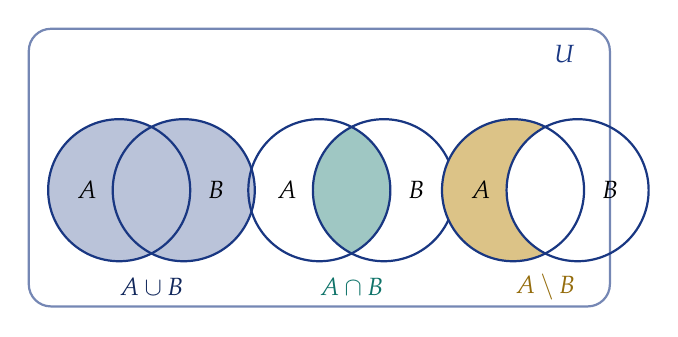
\begin{tikzpicture}[scale=0.82]
  % Universal set
  \draw[thick, royalblue!60, rounded corners=8pt]
    (-0.5,-1.8) rectangle (8.5,2.5);
  \node[royalblue, font=\small] at (7.8,2.1) {$U$};

  % ---- Union ----
  \begin{scope}[shift={(0,0)}]
    \fill[royalblue!30] (0.9,0) circle (1.1);
    \fill[royalblue!30] (1.9,0) circle (1.1);
    \draw[royalblue, thick] (0.9,0) circle (1.1);
    \draw[royalblue, thick] (1.9,0) circle (1.1);
    \node[font=\small] at (0.4,0) {$A$};
    \node[font=\small] at (2.4,0) {$B$};
    \node[royalblue!70!black, font=\small\bfseries] at (1.4,-1.5) {$A \cup B$};
  \end{scope}

  % ---- Intersection ----
  \begin{scope}[shift={(3.1,0)}]
    \begin{scope}
      \clip (0.9,0) circle (1.1);
      \fill[teal!40] (1.9,0) circle (1.1);
    \end{scope}
    \draw[royalblue, thick] (0.9,0) circle (1.1);
    \draw[royalblue, thick] (1.9,0) circle (1.1);
    \node[font=\small] at (0.4,0) {$A$};
    \node[font=\small] at (2.4,0) {$B$};
    \node[teal, font=\small\bfseries] at (1.4,-1.5) {$A \cap B$};
  \end{scope}

  % ---- Set difference ----
  \begin{scope}[shift={(6.1,0)}]
    \begin{scope}
      \clip (0.9,0) circle (1.1);
      \fill[gold!50] (0.9,0) circle (1.1);
      \fill[white] (1.9,0) circle (1.1);
    \end{scope}
    \draw[royalblue, thick] (0.9,0) circle (1.1);
    \draw[royalblue, thick] (1.9,0) circle (1.1);
    \node[font=\small] at (0.4,0) {$A$};
    \node[font=\small] at (2.4,0) {$B$};
    \node[gold!80!black, font=\small\bfseries] at (1.4,-1.5) {$A \setminus B$};
  \end{scope}
\end{tikzpicture}
\captionof*{figure}{\small Venn diagrams: Union (blue), Intersection (teal), Set Difference (gold)}
\end{center}

\begin{exbox}{Set Operations in Consumer Theory}
Let the universal set be $U = \R^2_+$ (all non-negative bundles of two goods). Let:
\[
  A = \{(x_1, x_2) \in \R^2_+ : x_1 + x_2 \leq 10\} \quad \text{(affordable at price 1, income 10)}
\]
\[
  B = \{(x_1, x_2) \in \R^2_+ : x_1 \geq 2 \text{ and } x_2 \geq 2\} \quad \text{(minimum requirements)}
\]
Then:
\begin{itemize}
  \item $A \cup B$ = bundles that are either affordable \emph{or} meet minimum requirements.
  \item $A \cap B = \{(x_1,x_2)\in\R^2_+: x_1+x_2\leq 10,\, x_1\geq 2,\, x_2\geq 2\}$ = affordable bundles that also meet minimum requirements (the relevant feasible set).
  \item $A \setminus B = \{(x_1,x_2)\in\R^2_+: x_1+x_2\leq 10\} \setminus B$ = affordable bundles that \emph{fail} to meet at least one minimum requirement.
  \item $A^c = \{(x_1,x_2)\in\R^2_+: x_1+x_2 > 10\}$ = unaffordable bundles.
\end{itemize}
\end{exbox}

\subsection{Laws of Set Algebra}

The following identities hold for all sets $A, B, C$ within universal set $U$:

\begin{thmbox}{Laws of Set Algebra}
\textbf{Commutativity}: $A \cup B = B \cup A$ \hfill $A \cap B = B \cap A$

\medskip
\textbf{Associativity}: $(A\cup B)\cup C = A\cup(B\cup C)$ \hfill $(A\cap B)\cap C = A\cap(B\cap C)$

\medskip
\textbf{Distributivity}: $A\cup(B\cap C) = (A\cup B)\cap(A\cup C)$ \hfill $A\cap(B\cup C) = (A\cap B)\cup(A\cap C)$

\medskip
\textbf{Identity}: $A\cup\emptyset = A$ \hfill $A\cap U = A$

\medskip
\textbf{Complement}: $A\cup A^c = U$ \hfill $A\cap A^c = \emptyset$

\medskip
\textbf{De Morgan's Laws}: $(A\cup B)^c = A^c\cap B^c$ \hfill $(A\cap B)^c = A^c\cup B^c$

\medskip
\textbf{Double complement}: $(A^c)^c = A$
\end{thmbox}

\begin{exbox}{Proving a Set Identity}
Prove: $A \setminus B = A \cap B^c$.

\textbf{Proof}: We show the two sets have identical membership.

($\subseteq$) Let $x \in A \setminus B$. Then $x \in A$ and $x \notin B$. Since $x \notin B$, we have $x \in B^c$. Therefore $x \in A \cap B^c$.

($\supseteq$) Let $x \in A \cap B^c$. Then $x \in A$ and $x \in B^c$, i.e.\ $x \in A$ and $x \notin B$. Therefore $x \in A \setminus B$.

Since each set is a subset of the other, $A \setminus B = A \cap B^c$. \qed
\end{exbox}
\newpage
\begin{exbox}{Applying De Morgan's Laws in Economics}
The \textbf{infeasible} region is the complement of the feasible set. Suppose the feasible set is:
\[
  F = \{x \in \R^n : g_1(x) \leq b_1\} \cap \{x \in \R^n : g_2(x) \leq b_2\} = G_1 \cap G_2
\]
By De Morgan's Law:
\[
  F^c = (G_1 \cap G_2)^c = G_1^c \cup G_2^c
\]
A bundle is \textit{infeasible} if and only if it violates \textit{at least one} constraint --- which is exactly $G_1^c \cup G_2^c$ (the union of the individual violation sets).
\end{exbox}

\subsection{Indexed Families of Sets}

When working with many sets simultaneously, we use indexed notation.

\begin{defbox}{Indexed Union and Intersection}
Let $\{A_\alpha\}_{\alpha \in I}$ be a family of sets indexed by $I$. Then:
\[
  \bigcup_{\alpha \in I} A_\alpha = \{x : x \in A_\alpha \text{ for some } \alpha \in I\}
\]
\[
  \bigcap_{\alpha \in I} A_\alpha = \{x : x \in A_\alpha \text{ for all } \alpha \in I\}
\]
\end{defbox}

\begin{exbox}{Nested Budget Sets}
For each income level $w > 0$, define the budget set $B_w = \{x \in \R^2_+ : p_1 x_1 + p_2 x_2 \leq w\}$ at fixed prices $(p_1, p_2)$.

\begin{itemize}
  \item $\displaystyle\bigcup_{w > 0} B_w = \R^2_+$\quad (any bundle is affordable at high enough income)
  \item $\displaystyle\bigcap_{w > 0} B_w = \{(0,0)\}$\quad (only the origin is affordable at every income level)
  \item If $w_1 < w_2$, then $B_{w_1} \subsetneq B_{w_2}$\quad (nested structure: richer budget sets contain poorer ones)
\end{itemize}
\end{exbox}

% ═══════════════════════════════════════════════════════════════════════════════
\section{Real Analysis: Intervals and Bounded Sets}
% ═══════════════════════════════════════════════════════════════════════════════

\subsection{Intervals in $\R$}

Intervals are the most important subsets of $\R$ in economic analysis. They model price ranges, income levels, time horizons, and parameter spaces.

\begin{defbox}{Types of Intervals}
For $a, b \in \R$ with $a < b$:
\begin{align*}
  [a,b]   &= \{x \in \R : a \leq x \leq b\} &\text{closed interval}\\
  (a,b)   &= \{x \in \R : a < x < b\}        &\text{open interval}\\
  [a,b)   &= \{x \in \R : a \leq x < b\}     &\text{half-open (closed at $a$)}\\
  (a,b]   &= \{x \in \R : a < x \leq b\}     &\text{half-open (closed at $b$)}\\
  [a,\infty) &= \{x \in \R : x \geq a\}       &\text{closed ray}\\
  (a,\infty) &= \{x \in \R : x > a\}          &\text{open ray}\\
  \R = (-\infty,\infty) & & \text{entire real line}
\end{align*}
\end{defbox}

\begin{defbox}{Bounded Sets}
A set $A \subseteq \R$ is:
\begin{itemize}
  \item \textbf{Bounded above} if there exists $M \in \R$ such that $x \leq M$ for all $x \in A$. The smallest such $M$ is the \textbf{supremum} $\sup A$.
  \item \textbf{Bounded below} if there exists $m \in \R$ such that $x \geq m$ for all $x \in A$. The largest such $m$ is the \textbf{infimum} $\inf A$.
  \item \textbf{Bounded} if it is bounded both above and below.
\end{itemize}
If $\sup A \in A$, it is called the \textbf{maximum} $\max A$. If $\inf A \in A$, it is called the \textbf{minimum} $\min A$.
\end{defbox}

\begin{exbox}{Supremum vs.\ Maximum}
\begin{enumerate}
  \item $A = [0,1]$: $\sup A = 1 = \max A$ and $\inf A = 0 = \min A$. (Both attained.)
  \item $B = (0,1)$: $\sup B = 1$ but $\max B$ does not exist (1 is not in $B$). Similarly $\inf B = 0$, $\min B$ does not exist.
  \item $C = \{1/n : n \in \N\} = \{1, 1/2, 1/3, \ldots\}$: $\sup C = 1 = \max C$, but $\inf C = 0$ and $\min C$ does not exist (0 is not in $C$).
\end{enumerate}

\textbf{Economic relevance}: In maximisation problems, we need $\sup$ when the maximum may not be attained (e.g.\ open feasible sets). The Extreme Value Theorem guarantees $\max$ exists when the domain is \textit{closed and bounded} (compact) and the objective is continuous.
\end{exbox}

\subsection{Open and Closed Sets in $\R^n$}

\begin{defbox}{Open Ball, Open Set, Closed Set}
In $\R^n$, the \textbf{open ball} of radius $r > 0$ centred at $x_0$ is:
\[
  B_r(x_0) = \{x \in \R^n : \|x - x_0\| < r\}
\]
A set $U \subseteq \R^n$ is \textbf{open} if for every $x \in U$, there exists $r > 0$ such that $B_r(x) \subseteq U$.

A set $F \subseteq \R^n$ is \textbf{closed} if its complement $F^c = \R^n \setminus F$ is open.
\end{defbox}

\begin{keybox}{Key Facts About Open and Closed Sets}
\begin{itemize}
  \item $\emptyset$ and $\R^n$ are both open \emph{and} closed.
  \item Finite intersections and arbitrary unions of open sets are open.
  \item Finite unions and arbitrary intersections of closed sets are closed.
  \item A set can be neither open nor closed (e.g.\ $[0,1)$ in $\R$).
  \item The budget set $\{x \geq 0 : p\cdot x \leq w\}$ is closed; the strict budget set $\{x \geq 0: p\cdot x < w\}$ is open.
\end{itemize}
\end{keybox}

% ═══════════════════════════════════════════════════════════════════════════════
\section{Functions: Core Concepts}
% ═══════════════════════════════════════════════════════════════════════════════

\subsection{Definition and Notation}

\begin{defbox}{Function}
A \textbf{function} $f$ from set $X$ to set $Y$, written $f: X \to Y$, is a rule that assigns to each element $x \in X$ \textbf{exactly one} element $f(x) \in Y$.

\begin{itemize}
  \item $X$ is the \textbf{domain} of $f$: $\dom(f) = X$
  \item $Y$ is the \textbf{codomain} of $f$
  \item $f(x)$ is the \textbf{image} (or value) of $x$ under $f$
  \item The \textbf{range} (image) of $f$: $\ran(f) = \img(f) = \{f(x) : x \in X\} \subseteq Y$
\end{itemize}
\end{defbox}

\begin{warnbox}{Functions are not just formulas}
A function is fully specified by its domain, codomain, and rule. The same formula with different domains defines different functions:
\begin{itemize}
  \item $f: \R \to \R$, $f(x) = x^2$ \hspace{1em}vs.\hspace{1em} $g: [0,\infty) \to \R$, $g(x) = x^2$
\end{itemize}
These are \textit{different} functions: $g$ is invertible while $f$ is not. Always state the domain explicitly.
\end{warnbox}

\begin{exbox}{Domain and Range in Economics}
Consider the inverse demand function $f: (0, \infty) \to (0, \infty)$, $f(Q) = \frac{100}{Q}$.
\begin{itemize}
  \item Domain: $\dom(f) = (0,\infty)$ (quantity must be strictly positive).
  \item Range: $\ran(f) = (0, \infty)$ (price takes all positive values).
\end{itemize}
Now consider a Cobb-Douglas production function $F: \R^2_+ \to \R_+$,
$F(K, L) = K^\alpha L^{1-\alpha}$ for $\alpha \in (0,1)$.
\begin{itemize}
  \item Domain: $\R^2_+$ (capital and labour must be non-negative).
  \item Range: $\R_+ = [0,\infty)$.
\end{itemize}
\end{exbox}

\subsection{Injective, Surjective, and Bijective Functions}

\begin{defbox}{Injective (One-to-One)}
$f: X \to Y$ is \textbf{injective} (one-to-one) if distinct inputs produce distinct outputs:
\[
  f(x_1) = f(x_2) \implies x_1 = x_2 \quad \text{(equivalently: } x_1 \neq x_2 \implies f(x_1) \neq f(x_2)\text{)}
\]
\end{defbox}

\begin{defbox}{Surjective (Onto)}
$f: X \to Y$ is \textbf{surjective} (onto) if every element of the codomain is hit by at least one input:
\[
  \forall y \in Y,\; \exists x \in X \st f(x) = y \quad \text{(equivalently: } \ran(f) = Y\text{)}
\]
\end{defbox}

\begin{defbox}{Bijective}
$f: X \to Y$ is \textbf{bijective} (a one-to-one correspondence) if it is both injective and surjective. Bijections set up a perfect pairing between $X$ and $Y$.
\end{defbox}

\medskip

\begin{center}
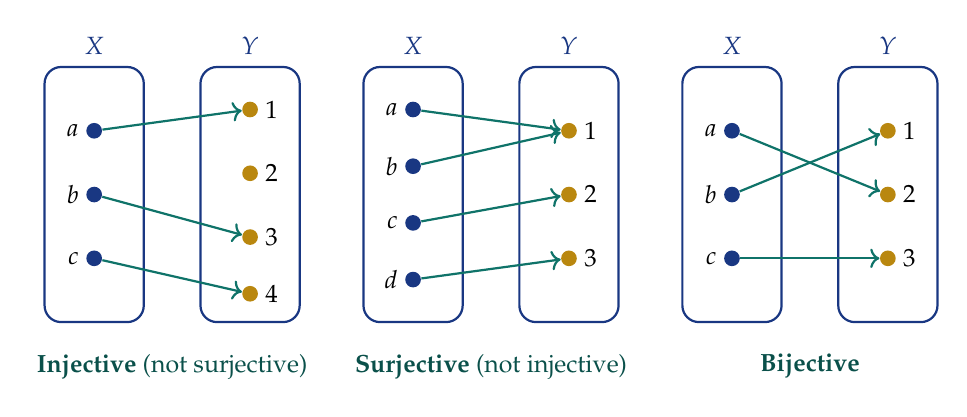
\begin{tikzpicture}[scale=0.9,
  every node/.style={font=\small},
  dot/.style={circle, fill, inner sep=2pt}]

  % ---------- Injective ----------
  \begin{scope}[shift={(0,0)}]
    \draw[royalblue, thick, rounded corners=6pt] (0,-0.3) rectangle (1.4,3.3);
    \draw[royalblue, thick, rounded corners=6pt] (2.2,-0.3) rectangle (3.6,3.3);
    \node[royalblue] at (0.7,3.6) {$X$};
    \node[royalblue] at (2.9,3.6) {$Y$};
    \foreach \y/\l in {2.4/a, 1.5/b, 0.6/c}{
      \node[dot,royalblue] (x\l) at (0.7,\y) {};
      \node[left=2pt] at (x\l) {$\l$};
    }
    \foreach \y/\l in {2.7/1, 1.8/2, 0.9/3, 0.1/4}{
      \node[dot,gold] (y\l) at (2.9,\y) {};
      \node[right=2pt] at (y\l) {$\l$};
    }
    \draw[->, thick, teal] (xa) -- (y1);
    \draw[->, thick, teal] (xb) -- (y3);
    \draw[->, thick, teal] (xc) -- (y4);
    \node[below=8pt, teal!70!black] at (1.8,-0.3) {\textbf{Injective} (not surjective)};
  \end{scope}

  % ---------- Surjective ----------
  \begin{scope}[shift={(4.5,0)}]
    \draw[royalblue, thick, rounded corners=6pt] (0,-0.3) rectangle (1.4,3.3);
    \draw[royalblue, thick, rounded corners=6pt] (2.2,-0.3) rectangle (3.6,3.3);
    \node[royalblue] at (0.7,3.6) {$X$};
    \node[royalblue] at (2.9,3.6) {$Y$};
    \foreach \y/\l in {2.7/a, 1.9/b, 1.1/c, 0.3/d}{
      \node[dot,royalblue] (x\l) at (0.7,\y) {};
      \node[left=2pt] at (x\l) {$\l$};
    }
    \foreach \y/\l in {2.4/1, 1.5/2, 0.6/3}{
      \node[dot,gold] (y\l) at (2.9,\y) {};
      \node[right=2pt] at (y\l) {$\l$};
    }
    \draw[->, thick, teal] (xa) -- (y1);
    \draw[->, thick, teal] (xb) -- (y1);
    \draw[->, thick, teal] (xc) -- (y2);
    \draw[->, thick, teal] (xd) -- (y3);
    \node[below=8pt, teal!70!black] at (1.8,-0.3) {\textbf{Surjective} (not injective)};
  \end{scope}

  % ---------- Bijective ----------
  \begin{scope}[shift={(9,0)}]
    \draw[royalblue, thick, rounded corners=6pt] (0,-0.3) rectangle (1.4,3.3);
    \draw[royalblue, thick, rounded corners=6pt] (2.2,-0.3) rectangle (3.6,3.3);
    \node[royalblue] at (0.7,3.6) {$X$};
    \node[royalblue] at (2.9,3.6) {$Y$};
    \foreach \y/\l in {2.4/a, 1.5/b, 0.6/c}{
      \node[dot,royalblue] (x\l) at (0.7,\y) {};
      \node[left=2pt] at (x\l) {$\l$};
    }
    \foreach \y/\l in {2.4/1, 1.5/2, 0.6/3}{
      \node[dot,gold] (y\l) at (2.9,\y) {};
      \node[right=2pt] at (y\l) {$\l$};
    }
    \draw[->, thick, teal] (xa) -- (y2);
    \draw[->, thick, teal] (xb) -- (y1);
    \draw[->, thick, teal] (xc) -- (y3);
    \node[below=8pt, teal!70!black] at (1.8,-0.3) {\textbf{Bijective}};
  \end{scope}
\end{tikzpicture}
\end{center}

\begin{exbox}{Classifying Economic Functions}
\begin{enumerate}
  \item $f: \R \to \R$, $f(x) = 2x + 3$. \textbf{Bijective.}
    \begin{itemize}
      \item Injective: $f(x_1)=f(x_2) \Rightarrow 2x_1+3=2x_2+3 \Rightarrow x_1=x_2$. \checkmark
      \item Surjective: for any $y$, $x=(y-3)/2\in\R$ satisfies $f(x)=y$. \checkmark
    \end{itemize}
  \item $g: \R \to \R$, $g(x) = x^2$. \textbf{Neither injective nor surjective.}
    \begin{itemize}
      \item Not injective: $g(-2)=g(2)=4$ but $-2\neq 2$.
      \item Not surjective: $-1 \in \R$ but $g(x)=x^2\geq 0>-1$ for all $x$, so no $x$ maps to $-1$.
    \end{itemize}
  \item $h: [0,\infty) \to [0,\infty)$, $h(x) = x^2$. \textbf{Bijective.}
    \begin{itemize}
      \item Injective: $h(x_1)=h(x_2)$ and $x_1,x_2\geq 0 \Rightarrow x_1=x_2$. \checkmark
      \item Surjective: for any $y\geq 0$, $x=\sqrt{y}\geq 0$ satisfies $h(x)=y$. \checkmark
    \end{itemize}
  \item Profit function $\pi: \R_+ \to \R$, $\pi(q) = pq - cq^2$. \textbf{Not injective} (two output levels can yield the same profit), \textbf{not surjective onto} $\R$ from $\R_+$ (range is $(-\infty, p^2/(4c)]$).
\end{enumerate}
\end{exbox}

\subsection{Image and Pre-image}

\begin{defbox}{Image and Pre-image of Sets}
Let $f: X \to Y$, $A \subseteq X$, and $B \subseteq Y$.

The \textbf{image} of $A$ under $f$:
\[
  f(A) = \{f(x) : x \in A\} \subseteq Y
\]
The \textbf{pre-image} (inverse image) of $B$ under $f$:
\[
  f^{-1}(B) = \{x \in X : f(x) \in B\} \subseteq X
\]
Note: $f^{-1}(B)$ is defined for any function $f$ (even non-invertible ones); it simply collects all inputs mapping into $B$.
\end{defbox}

\begin{thmbox}{Properties of Images and Pre-images}
Let $f: X \to Y$, $A_1, A_2 \subseteq X$, and $B_1, B_2 \subseteq Y$. Then:
\begin{align*}
  f(A_1 \cup A_2) &= f(A_1) \cup f(A_2) \\
  f(A_1 \cap A_2) &\subseteq f(A_1) \cap f(A_2) \quad \text{(equality holds if $f$ is injective)}\\
  f^{-1}(B_1 \cup B_2) &= f^{-1}(B_1) \cup f^{-1}(B_2) \\
  f^{-1}(B_1 \cap B_2) &= f^{-1}(B_1) \cap f^{-1}(B_2) \\
  f^{-1}(B^c) &= \bigl(f^{-1}(B)\bigr)^c
\end{align*}
Pre-images behave better than images under set operations.
\end{thmbox}

\begin{exbox}{Pre-image in Welfare Analysis}
Let $f: \R_+ \to \R$ be a utility function $f(x) = \ln(1+x)$. The regulator defines a welfare threshold $B = [\ln 2, \infty)$ (utility at least $\ln 2$).

The pre-image is:
\[
  f^{-1}(B) = \{x \geq 0 : \ln(1+x) \geq \ln 2\} = \{x \geq 0 : 1+x \geq 2\} = [1, \infty)
\]
Interpretation: consumers with consumption $x \geq 1$ achieve the welfare threshold. The pre-image gives the \emph{set of inputs that are socially adequate}.
\end{exbox}


\newpage %═══════════════════════════════════════════════════════════════════════════════
\section{Function Composition and Inverse Functions}
% ═══════════════════════════════════════════════════════════════════════════════

\subsection{Composition of Functions}

\begin{defbox}{Composition}
Let $f: X \to Y$ and $g: Y \to Z$. The \textbf{composition} $g \circ f: X \to Z$ is defined by:
\[
  (g \circ f)(x) = g(f(x)) \quad \forall x \in X
\]
\end{defbox}

\begin{warnbox}{Order of Composition}
$g \circ f$ means ``first apply $f$, then apply $g$''. This is read right-to-left. In general, $g \circ f \neq f \circ g$ (composition is \textbf{not} commutative).
\end{warnbox}

\begin{exbox}{Composition in Macroeconomics}
Let $Y$ be GDP, $U$ be unemployment, and $I$ be inflation:
\[
  f: \text{GDP} \to \text{Unemployment},\quad f(Y) = \bar{u} - \beta(Y - \bar{Y}) \quad \text{(Okun's Law)}
\]
\[
  g: \text{Unemployment} \to \text{Inflation},\quad g(U) = \pi^e - \gamma(U - \bar{u}) \quad \text{(Phillips Curve)}
\]
The composed function $g \circ f: \text{GDP} \to \text{Inflation}$:
\[
  (g \circ f)(Y) = g(f(Y)) = \pi^e - \gamma\bigl(\bar{u} - \beta(Y-\bar{Y}) - \bar{u}\bigr) = \pi^e + \gamma\beta(Y - \bar{Y})
\]
This is the ``aggregate supply curve'': higher output above potential raises inflation via the unemployment channel.
\end{exbox}

\begin{thmbox}{Properties of Composition}
Let $f: X\to Y$, $g: Y\to Z$, $h: Z\to W$. Then:
\begin{enumerate}
  \item \textbf{Associativity}: $h\circ(g\circ f) = (h\circ g)\circ f$
  \item If $f$ and $g$ are injective, then $g\circ f$ is injective.
  \item If $f$ and $g$ are surjective, then $g\circ f$ is surjective.
  \item If $f$ and $g$ are bijective, then $g\circ f$ is bijective and $(g\circ f)^{-1} = f^{-1}\circ g^{-1}$.
\end{enumerate}
\end{thmbox}

\subsection{Inverse Functions}

\begin{defbox}{Inverse Function}
Let $f: X \to Y$ be a bijection. The \textbf{inverse function} $f^{-1}: Y \to X$ is the unique function satisfying:
\[
  f^{-1}(f(x)) = x \;\;\forall x \in X \quad \text{and} \quad f(f^{-1}(y)) = y \;\;\forall y \in Y
\]
Equivalently, $f^{-1} \circ f = \mathrm{id}_X$ and $f \circ f^{-1} = \mathrm{id}_Y$, where $\mathrm{id}$ denotes the identity function.
\end{defbox}

\begin{keybox}{When Does an Inverse Exist?}
$f: X \to Y$ has an inverse $f^{-1}: Y \to X$ if and only if $f$ is \textbf{bijective}. For real-valued functions:
\begin{itemize}
  \item A \textbf{strictly monotone} function $f: I \to \R$ on an interval $I$ is injective.
  \item The inverse of a strictly increasing function is strictly increasing.
  \item The inverse of a strictly decreasing function is strictly decreasing.
  \item Geometrically: the graph of $f^{-1}$ is the reflection of the graph of $f$ across the line $y = x$.
\end{itemize}
\end{keybox}

\begin{exbox}{Inverse Functions in Economics}

\textbf{1. Demand and Inverse Demand.}
Let $Q = D(P) = 120 - 2P$ be the demand function ($P \geq 0$, $Q \geq 0$).
\begin{itemize}
  \item Domain of $D$: $[0, 60]$ (prices giving non-negative quantity).
  \item Inverse: solve for $P$: $Q = 120 - 2P \Rightarrow P = 60 - Q/2$.
  \item So $D^{-1}(Q) = P(Q) = 60 - Q/2$ is the inverse demand.
  \item This is economically meaningful: $P(Q)$ gives the maximum price consumers pay for $Q$ units.
\end{itemize}

\textbf{2. Expenditure and Indirect Utility.}
The expenditure function $e(p, u)$ and indirect utility function $v(p, w)$ are inverses of each other in the utility argument: $e(p, v(p,w)) = w$ and $v(p, e(p,u)) = u$. This is Shephard's duality.

\textbf{3. Production.} If $F: [0,\infty) \to [0,\infty)$, $F(L) = \sqrt{L}$, then $F^{-1}(Q) = Q^2$ gives the labour required to produce $Q$ units.
\end{exbox}

\begin{exbox}{Finding Inverse Functions: Step-by-Step}
Find the inverse of $f(x) = \dfrac{3x-1}{x+2}$ (where $x \neq -2$).

\textbf{Step 1}: Write $y = \dfrac{3x-1}{x+2}$ and solve for $x$.

\textbf{Step 2}: $y(x+2) = 3x-1 \Rightarrow xy + 2y = 3x - 1 \Rightarrow xy - 3x = -2y - 1$

\textbf{Step 3}: $x(y-3) = -2y-1 \Rightarrow x = \dfrac{-2y-1}{y-3} = \dfrac{2y+1}{3-y}$

\textbf{Step 4}: So $f^{-1}(y) = \dfrac{2y+1}{3-y}$, defined for $y \neq 3$.

\textbf{Verify}: $f(f^{-1}(y)) = f\!\left(\dfrac{2y+1}{3-y}\right) = \dfrac{3\cdot\frac{2y+1}{3-y}-1}{\frac{2y+1}{3-y}+2} = \dfrac{\frac{6y+3-(3-y)}{3-y}}{\frac{2y+1+2(3-y)}{3-y}} = \dfrac{7y}{7} = y$ \checkmark
\end{exbox}

% ═══════════════════════════════════════════════════════════════════════════════
\section{Types of Functions in Economic Analysis}
% ═══════════════════════════════════════════════════════════════════════════════

\subsection{Monotone Functions}

\begin{defbox}{Monotone Functions}
A function $f: X \subseteq \R \to \R$ is:
\begin{itemize}
  \item \textbf{Strictly increasing}: $x_1 < x_2 \Rightarrow f(x_1) < f(x_2)$
  \item \textbf{Weakly increasing}: $x_1 < x_2 \Rightarrow f(x_1) \leq f(x_2)$
  \item \textbf{Strictly decreasing}: $x_1 < x_2 \Rightarrow f(x_1) > f(x_2)$
  \item \textbf{Weakly decreasing}: $x_1 < x_2 \Rightarrow f(x_1) \geq f(x_2)$
\end{itemize}
$f$ is \textbf{monotone} if it is either weakly increasing or weakly decreasing. Strictly monotone functions are always injective.
\end{defbox}

\subsection{Convex and Concave Functions}

\begin{defbox}{Convex and Concave Functions}
A function $f: C \to \R$ on a convex set $C \subseteq \R^n$ is:

\textbf{Convex} if for all $x, y \in C$ and $\lambda \in [0,1]$:
\[
  f(\lambda x + (1-\lambda)y) \leq \lambda f(x) + (1-\lambda)f(y)
\]
\textbf{Concave} if for all $x, y \in C$ and $\lambda \in [0,1]$:
\[
  f(\lambda x + (1-\lambda)y) \geq \lambda f(x) + (1-\lambda)f(y)
\]
$f$ is \textbf{strictly convex} (resp.\ \textbf{strictly concave}) if the inequality is strict for $\lambda \in (0,1)$ and $x \neq y$.
\end{defbox}

\begin{center}
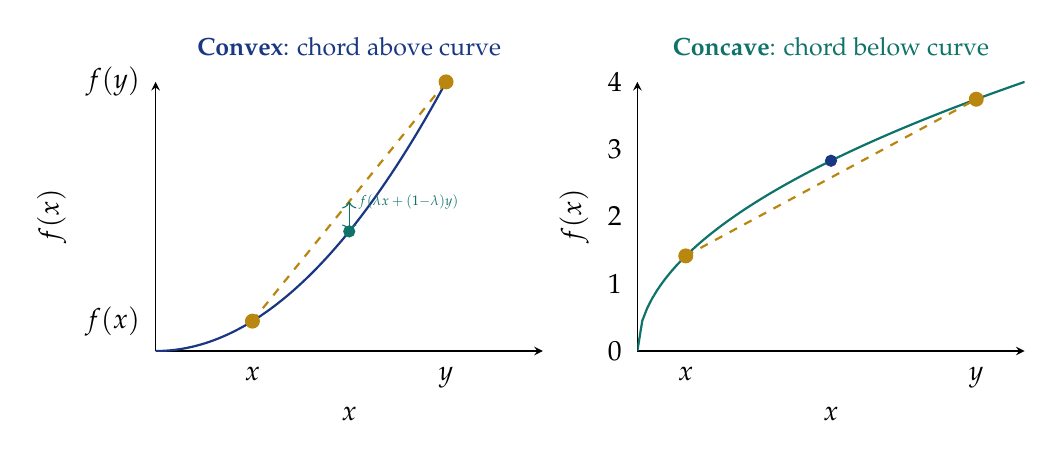
\begin{tikzpicture}
  \begin{axis}[
    name=ax1, width=6.5cm, height=5cm,
    axis lines=left,
    xlabel={$x$}, ylabel={$f(x)$},
    xmin=0, xmax=4, ymin=0, ymax=9,
    xtick={1,3}, xticklabels={$x$,$y$},
    ytick={1,9},yticklabels={$f(x)$,$f(y)$},
    title={\small\textbf{Convex}: chord above curve},
    title style={color=royalblue},
    tick style={draw=none},
    grid=none,
  ]
    \addplot[thick, royalblue, domain=0:4, samples=80] {x^2};
    \addplot[thick, gold, dashed] coordinates {(1,1)(3,9)};
    \addplot[only marks, mark=*, mark size=2.5pt, gold]
      coordinates {(1,1)(3,9)};
    \addplot[only marks, mark=*, mark size=2pt, teal]
      coordinates {(2,4)};
    \draw[teal,<->] (axis cs:2,4) -- (axis cs:2,5) node[right,font=\tiny]{$f(\lambda x+(1{-}\lambda)y)$};
  \end{axis}

  \begin{axis}[
    name=ax2, at={(ax1.east)}, anchor=west, xshift=1.2cm,
    width=6.5cm, height=5cm,
    axis lines=left,
    xlabel={$x$}, ylabel={$f(x)$},
    xmin=0, xmax=4, ymin=0, ymax=4,
    xtick={0.5,3.5}, xticklabels={$x$,$y$},
    title={\small\textbf{Concave}: chord below curve},
    title style={color=teal},
    tick style={draw=none},
    grid=none,
  ]
    \addplot[thick, teal, domain=0:4, samples=80] {sqrt(4*x)};
    \addplot[thick, gold, dashed] coordinates {(0.5,1.414)(3.5,3.742)};
    \addplot[only marks, mark=*, mark size=2.5pt, gold]
      coordinates {(0.5,1.414)(3.5,3.742)};
    \addplot[only marks, mark=*, mark size=2pt, royalblue]
      coordinates {(2,2.828)};
  \end{axis}
\end{tikzpicture}
\end{center}

\begin{keybox}{Concavity in Economics}
\begin{itemize}
  \item \textbf{Utility functions} are typically assumed concave --- this captures diminishing marginal utility and gives rise to risk aversion.
  \item \textbf{Production functions} are typically concave in inputs --- this captures diminishing marginal product.
  \item \textbf{Cost functions} are convex in output --- this reflects increasing marginal cost.
  \item If $f$ is concave and differentiable, then $f''(x) \leq 0$ for all $x$.
  \item Any local maximum of a concave function is a global maximum --- critical for optimisation.
\end{itemize}
\end{keybox}

\begin{exbox}{Testing Convexity and Concavity}
\begin{enumerate}
  \item $f(x) = x^2$, $f''(x) = 2 > 0$: \textbf{strictly convex}.
  \item $f(x) = \ln x$ for $x > 0$, $f''(x) = -1/x^2 < 0$: \textbf{strictly concave}.
  \item $f(x) = e^x$, $f''(x) = e^x > 0$: \textbf{strictly convex}.
  \item Cobb-Douglas $F(K,L) = K^\alpha L^\beta$ with $\alpha+\beta < 1$: \textbf{concave} (diminishing returns to scale).

  \textbf{Verify} using the definition for (2): For $x, y > 0$ and $\lambda \in [0,1]$, we need $\ln(\lambda x + (1-\lambda)y) \geq \lambda\ln x + (1-\lambda)\ln y = \ln(x^\lambda y^{1-\lambda})$.

  This says $\lambda x + (1-\lambda)y \geq x^\lambda y^{1-\lambda}$, which is the \textbf{AM-GM inequality} --- a classical result. \checkmark
\end{enumerate}
\end{exbox}

\subsection{Homogeneous Functions}

\begin{defbox}{Homogeneous Function}
A function $f: \R^n_+ \to \R$ is \textbf{homogeneous of degree $k$} if for all $t > 0$ and all $x \in \R^n_+$:
\[
  f(tx) = t^k f(x)
\]
\end{defbox}

\begin{thmbox}{Euler's Theorem}
If $f: \R^n_+ \to \R$ is differentiable and homogeneous of degree $k$, then:
\[
  \sum_{i=1}^n x_i \frac{\partial f}{\partial x_i}(x) = k \cdot f(x)
\]
\end{thmbox}

\begin{exbox}{Homogeneity in Producer Theory}
\begin{itemize}
  \item \textbf{Constant returns to scale}: $F(tK, tL) = tF(K,L)$ --- homogeneous of degree 1.\\
    Euler: $K \cdot F_K + L \cdot F_L = F(K,L)$ --- the sum of marginal products weighted by inputs equals total output (the zero-profit condition for competitive firms).
  \item \textbf{Cobb-Douglas} $F(K,L) = K^\alpha L^\beta$:
    $F(tK,tL) = (tK)^\alpha(tL)^\beta = t^{\alpha+\beta}K^\alpha L^\beta = t^{\alpha+\beta}F(K,L)$.\\
    Degree $= \alpha+\beta$: IRS if $>1$, CRS if $= 1$, DRS if $<1$.
  \item \textbf{Demand functions}: Walrasian demand $x(p,w)$ is homogeneous of degree 0 in $(p,w)$ --- doubling all prices and income leaves demand unchanged (no money illusion).
\end{itemize}
\end{exbox}

\newpage
% ═══════════════════════════════════════════════════════════════════════════════
\section{Practice Questions}
% ═══════════════════════════════════════════════════════════════════════════════

\subsection{Section A: Sets and Set Operations}

\begin{enumerate}[label=\textbf{A\arabic*.}, leftmargin=2.5em]

  \item \textbf{(Set Builder Notation)} Write each of the following sets in set-builder notation and determine whether it is finite or infinite:
  \begin{enumerate}[label=(\alph*)]
    \item The set of all even natural numbers less than 20.
    \item The set of all real numbers whose square is less than 16.
    \item The set of all prices in $[0, 100]$ that make demand positive, given $D(P) = 50 - P$.
  \end{enumerate}

  \item \textbf{(Set Operations)} Let $U = \{1,2,3,4,5,6,7,8,9,10\}$, $A = \{1,2,3,4,5\}$, $B = \{3,4,5,6,7\}$, and $C = \{5,6,7,8,9\}$. Compute:
  \begin{enumerate}[label=(\alph*)]
    \item $A \cup B$ \quad (b) $A \cap B$ \quad (c) $A \setminus B$ \quad (d) $B \setminus A$ \quad (e) $(A \cup B)^c$ \quad (f) $A \cap B \cap C$ \quad (g) $A \cup (B \cap C)$
  \end{enumerate}

  \item \textbf{(Power Set)} Find the power set of $A = \{x, y\}$. How many elements does $\powerset(\powerset(A))$ have?

  \item \textbf{(Cartesian Product)} Let $A = \{1, 2\}$ and $B = \{a, b, c\}$. List all elements of $A \times B$ and $B \times A$. Are they equal?

  \item \textbf{(De Morgan's Laws)} Verify De Morgan's Law $(A \cup B)^c = A^c \cap B^c$ using $U = \{1,\ldots,8\}$, $A=\{1,2,3,4\}$, $B=\{3,4,5,6\}$.

  \item \textbf{(Economic Application)} A consumer has income $w = 100$ and faces prices $p_1 = 2$, $p_2 = 5$. Define:
    \[A = \{(x_1,x_2)\in\R^2_+ : 2x_1 + 5x_2 \leq 100\}\]
    \[B = \{(x_1,x_2)\in\R^2_+ : x_1 \geq 10\}\]
    Describe $A \cap B$ geometrically. What does this set represent economically?

  \item \textbf{(Proof)} Prove the distributive law: $A \cap (B \cup C) = (A \cap B) \cup (A \cap C)$ using the element-chasing method.

  \item \textbf{(Supremum and Infimum)} For each set, find $\sup$, $\inf$, and state whether $\max$ and $\min$ exist:
  \begin{enumerate}[label=(\alph*)]
    \item $A = \left\{\frac{n}{n+1} : n \in \N\right\}$
    \item $B = (-3, 5]$
    \item $C = \{x \in \R : x^2 < 9\}$
    \item $D = \{x \in \R : x^3 \leq 8\}$
  \end{enumerate}
\end{enumerate}
\newpage
\subsection{Section B: Functions}

\begin{enumerate}[label=\textbf{B\arabic*.}, leftmargin=2.5em]

  \item \textbf{(Domain and Range)} Find the natural domain and range of:
  \begin{enumerate}[label=(\alph*)]
    \item $f(x) = \sqrt{9 - x^2}$
    \item $g(x) = \dfrac{x-1}{x^2-4}$
    \item $h(x) = \ln(x^2 - 1)$
    \item $k(x,y) = \sqrt{x} + \sqrt{y}$ (treat as a function from $\R^2$)
  \end{enumerate}

  \item \textbf{(Injectivity and Surjectivity)} For each function, determine whether it is injective, surjective, bijective, or none:
  \begin{enumerate}[label=(\alph*)]
    \item $f: \R \to \R$, $f(x) = 3x - 7$
    \item $g: \R \to \R$, $g(x) = x^3 - x$
    \item $h: \R \to \R^+$, $h(x) = e^x$
    \item $k: [0,\pi] \to [-1,1]$, $k(x) = \cos x$
    \item $\ell: \R_+ \to \R_+$, $\ell(x) = x^3$
  \end{enumerate}

  \item \textbf{(Inverse Functions)} Find the inverse of each function and state its domain:
  \begin{enumerate}[label=(\alph*)]
    \item $f(x) = 5x + 3$
    \item $g(x) = \dfrac{x+1}{x-2}$, $x \neq 2$
    \item $h(x) = e^{2x-1}$
    \item $k(x) = x^3 + 2$ on $\R$
  \end{enumerate}

  \item \textbf{(Composition)} Let $f(x) = 2x^2 - 1$ and $g(x) = \sqrt{x+3}$ (defined on $[-3,\infty)$). Compute:
  \begin{enumerate}[label=(\alph*)]
    \item $(g \circ f)(x)$ and state its domain.
    \item $(f \circ g)(x)$ and state its domain.
    \item $(g \circ f)(2)$ and $(f \circ g)(1)$.
    \item Are $g \circ f$ and $f \circ g$ equal? What does this illustrate?
  \end{enumerate}

  \item \textbf{(Pre-image)} Let $f:\R\to\R$, $f(x) = x^2 - 4$. Find:
  \begin{enumerate}[label=(\alph*)]
    \item $f^{-1}(\{0\})$\quad (b) $f^{-1}([-4, 0])$\quad (c) $f^{-1}((0,5])$\quad (d) $f^{-1}(\{-5\})$
  \end{enumerate}
\newpage
  \item \textbf{(Homogeneity)} Determine whether each function is homogeneous, and if so, find the degree:
  \begin{enumerate}[label=(\alph*)]
    \item $f(K,L) = 3K^{0.4}L^{0.6}$
    \item $g(x,y) = x^2 + xy + y^2$
    \item $h(x,y) = \dfrac{x^2 y}{x^3 + y^3}$
    \item $k(x,y) = x + y + 1$
  \end{enumerate}

  \item \textbf{(Concavity and Convexity)} Determine whether each function is convex, concave, or neither:
  \begin{enumerate}[label=(\alph*)]
    \item $f(x) = x^4$ on $\R$
    \item $g(x) = x^3$ on $\R$
    \item $h(x) = -2x^2 + 4x - 1$ on $\R$
    \item $k(x) = |x|$ on $\R$
  \end{enumerate}

  \item \textbf{(Economic Application --- Full Question)} A monopolist faces inverse demand $P(Q) = 100 - 2Q$ and has total cost $C(Q) = Q^2 + 10Q + 50$.
  \begin{enumerate}[label=(\alph*)]
    \item Define the profit function $\pi(Q)$ and state its domain.
    \item Find the range of $\pi$.
    \item Is $\pi$ concave? Justify.
    \item Find the profit-maximising quantity and maximum profit.
    \item Find $\pi^{-1}(\{0\})$ (the break-even quantities) and interpret.
  \end{enumerate}
\end{enumerate}

\newpage
% ═══════════════════════════════════════════════════════════════════════════════
\section{Full Solutions}
% ═══════════════════════════════════════════════════════════════════════════════

\subsection{Solutions: Section A}

\begin{solbox}
\textbf{A1. Set Builder Notation}

\textbf{(a)} Even natural numbers less than 20:
\[A = \{x \in \N : x \text{ is even and } x < 20\} = \{2, 4, 6, 8, 10, 12, 14, 16, 18\}.\quad\text{Finite (9 elements).}\]

\textbf{(b)} Real numbers with $x^2 < 16$:
\[B = \{x \in \R : x^2 < 16\} = \{x \in \R : |x| < 4\} = (-4, 4).\quad\text{Infinite.}\]

\textbf{(c)} Prices with $D(P) = 50 - P > 0$ and $P \in [0,100]$:

$D(P) > 0 \Rightarrow P < 50$. Combined with $P \in [0,100]$:
\[C = \{P \in [0,100] : 50 - P > 0\} = [0, 50).\quad\text{Infinite.}\]
\end{solbox}

\begin{solbox}
\textbf{A2. Set Operations}

With $U=\{1,\ldots,10\}$, $A=\{1,2,3,4,5\}$, $B=\{3,4,5,6,7\}$, $C=\{5,6,7,8,9\}$:

\textbf{(a)} $A \cup B = \{1,2,3,4,5,6,7\}$

\textbf{(b)} $A \cap B = \{3,4,5\}$

\textbf{(c)} $A \setminus B = \{1,2\}$\quad (elements in $A$ not in $B$)

\textbf{(d)} $B \setminus A = \{6,7\}$\quad (elements in $B$ not in $A$)

\textbf{(e)} $(A \cup B)^c = U \setminus \{1,2,3,4,5,6,7\} = \{8,9,10\}$

\textbf{(f)} $A \cap B \cap C = \{3,4,5\} \cap \{5,6,7,8,9\} = \{5\}$

\textbf{(g)} $B \cap C = \{5,6,7\}$, so $A \cup (B \cap C) = \{1,2,3,4,5\} \cup \{5,6,7\} = \{1,2,3,4,5,6,7\}$

\textbf{Check distributivity}: $A \cup (B \cap C) = (A \cup B) \cap (A \cup C)$.
$A \cup B = \{1,2,3,4,5,6,7\}$, $A \cup C = \{1,2,3,4,5,6,7,8,9\}$.
$(A\cup B)\cap(A\cup C) = \{1,2,3,4,5,6,7\}$. \checkmark
\end{solbox}

\begin{solbox}
\textbf{A3. Power Set}

$A = \{x, y\}$, so $|A|=2$ and $|\powerset(A)| = 2^2 = 4$:
\[\powerset(A) = \{\emptyset, \{x\}, \{y\}, \{x,y\}\}\]
Now $|\powerset(A)| = 4$, so $|\powerset(\powerset(A))| = 2^4 = \mathbf{16}$.
\end{solbox}

\begin{solbox}
\textbf{A4. Cartesian Product}

$A\times B = \{(1,a),(1,b),(1,c),(2,a),(2,b),(2,c)\}$\quad ($|A\times B| = 2\times 3 = 6$ elements)

$B\times A = \{(a,1),(a,2),(b,1),(b,2),(c,1),(c,2)\}$\quad ($|B\times A| = 3\times 2 = 6$ elements)

$A\times B \neq B\times A$: the pairs are ordered differently; e.g.\ $(1,a)\in A\times B$ but $(1,a)\notin B\times A$ since $1\notin B$. In general $A\times B = B\times A$ only if $A = B$.
\end{solbox}

\begin{solbox}
\textbf{A5. De Morgan's Law Verification}

$U=\{1,\ldots,8\}$, $A=\{1,2,3,4\}$, $B=\{3,4,5,6\}$.

\textbf{Left side}: $A\cup B = \{1,2,3,4,5,6\}$, so $(A\cup B)^c = \{7,8\}$.

\textbf{Right side}: $A^c = \{5,6,7,8\}$, $B^c = \{1,2,7,8\}$, so $A^c\cap B^c = \{7,8\}$.

$(A\cup B)^c = A^c \cap B^c = \{7,8\}$. \checkmark
\end{solbox}

\begin{solbox}
\textbf{A6. Budget Set Intersection}

$A = \{(x_1,x_2)\in\R^2_+ : 2x_1+5x_2\leq 100\}$ is the full budget set (triangle with vertices $(0,0)$, $(50,0)$, $(0,20)$).

$B = \{(x_1,x_2)\in\R^2_+ : x_1 \geq 10\}$ is the closed half-plane to the right of $x_1=10$.

$A\cap B = \{(x_1,x_2)\in\R^2_+ : 2x_1+5x_2\leq 100,\ x_1\geq 10\}$

Geometrically: the budget triangle \emph{truncated} by the vertical line $x_1=10$. It is a quadrilateral with vertices $(10,0)$, $(50,0)$, $(0,20)$... wait --- at $x_1=10$: $2(10)+5x_2\leq 100 \Rightarrow x_2\leq 16$. So the binding vertices are $(10,0)$, $(50,0)$, and $(10,16)$.

\textbf{Economic interpretation}: affordable bundles that contain \emph{at least 10 units of good 1} (perhaps a minimum consumption requirement or a rationing constraint). This is the feasible set when the consumer is forced to consume at least 10 units of good 1.
\end{solbox}

\begin{solbox}
\textbf{A7. Proof of Distributive Law}

We prove $A\cap(B\cup C) = (A\cap B)\cup(A\cap C)$ by element-chasing.

\textbf{($\subseteq$)}: Let $x \in A\cap(B\cup C)$. Then $x\in A$ and $x\in B\cup C$.

\textit{Case 1}: $x\in B$. Then $x\in A$ and $x\in B$, so $x\in A\cap B\subseteq (A\cap B)\cup(A\cap C)$.

\textit{Case 2}: $x\in C$. Then $x\in A$ and $x\in C$, so $x\in A\cap C\subseteq (A\cap B)\cup(A\cap C)$.

In either case, $x\in(A\cap B)\cup(A\cap C)$.

\textbf{($\supseteq$)}: Let $x\in(A\cap B)\cup(A\cap C)$.

\textit{Case 1}: $x\in A\cap B$. Then $x\in A$ and $x\in B\subseteq B\cup C$, so $x\in A\cap(B\cup C)$.

\textit{Case 2}: $x\in A\cap C$. Then $x\in A$ and $x\in C\subseteq B\cup C$, so $x\in A\cap(B\cup C)$.

Since $A\cap(B\cup C)\subseteq(A\cap B)\cup(A\cap C)$ and $(A\cap B)\cup(A\cap C)\subseteq A\cap(B\cup C)$, equality holds. \qed
\end{solbox}

\begin{solbox}
\textbf{A8. Supremum and Infimum}

\textbf{(a)} $A=\left\{\frac{n}{n+1}:n\in\N\right\} = \left\{\frac{1}{2},\frac{2}{3},\frac{3}{4},\ldots\right\}$

The sequence $n/(n+1)$ is strictly increasing and approaches 1. So $\sup A = 1$ (not attained: $n/(n+1)<1$ for all $n$, so $\max A$ does not exist). $\inf A = \min A = \frac{1}{2}$ (attained at $n=1$).

\textbf{(b)} $B=(-3,5]$: $\inf B = -3$ (not attained, $\min B$ DNE); $\sup B = \max B = 5$.

\textbf{(c)} $C=\{x\in\R:x^2<9\} = (-3,3)$: $\inf C = -3$ (DNE); $\sup C = 3$ (DNE). Neither $\min$ nor $\max$ exists.

\textbf{(d)} $D=\{x\in\R:x^3\leq 8\} = (-\infty,2]$: $\sup D = \max D = 2$. $D$ is unbounded below: $\inf D = -\infty$ (no infimum in $\R$).
\end{solbox}

\subsection{Solutions: Section B}

\begin{solbox}
\textbf{B1. Domain and Range}

\textbf{(a)} $f(x)=\sqrt{9-x^2}$: need $9-x^2\geq 0$, i.e.\ $x^2\leq 9$, i.e.\ $x\in[-3,3]$.

Range: $f(x)\geq 0$ and $f(0)=3$, so range $=[0,3]$.

\textbf{(b)} $g(x)=\frac{x-1}{x^2-4}=\frac{x-1}{(x-2)(x+2)}$: need $x\neq\pm 2$.

Domain $= \R\setminus\{-2,2\}$. Range: $g$ takes all real values except... at $x=1$, $g(1)=0$. Analysis shows range $=\R$ (every value achieved by continuity and the behaviour near the poles).

\textbf{(c)} $h(x)=\ln(x^2-1)$: need $x^2-1>0$, i.e.\ $|x|>1$.

Domain $=(-\infty,-1)\cup(1,\infty)$. As $|x|\to 1^+$, $\ln(x^2-1)\to-\infty$; as $|x|\to\infty$, $\ln(x^2-1)\to\infty$. Range $=\R=(-\infty,\infty)$.

\textbf{(d)} $k(x,y)=\sqrt{x}+\sqrt{y}$: need $x\geq 0$ and $y\geq 0$.

Domain $= \R^2_+ = [0,\infty)^2$. Range: $k(x,y)\geq 0$ always; for any $z\geq 0$, take $x=z^2$, $y=0$: $k(z^2,0)=z$. Range $=[0,\infty)$.
\end{solbox}

\begin{solbox}
\textbf{B2. Injectivity and Surjectivity}

\textbf{(a)} $f(x)=3x-7$: \textbf{Bijective.}

Injective: $3x_1-7=3x_2-7 \Rightarrow x_1=x_2$. \checkmark

Surjective: for any $y\in\R$, $x=(y+7)/3$ gives $f(x)=y$. \checkmark

\textbf{(b)} $g(x)=x^3-x=x(x-1)(x+1)$: \textbf{Neither.}

Not injective: $g(0)=0=g(1) \cdot$... let's check: $g(0)=0$, $g(-1)=(-1)(0) = 0$ wait: $g(-1)=(-1)(-2)(0)=0$. So $g(0)=g(-1)=0$ with $0\neq -1$. Not injective.

Not surjective? Actually it IS surjective since $\lim_{x\to\pm\infty}g(x)=\pm\infty$ and $g$ is continuous, so by IVT every value in $\R$ is achieved. So $g$ is \textbf{surjective but not injective}.

\textbf{(c)} $h:\R\to\R^+$, $h(x)=e^x$: \textbf{Bijective.}

Injective: $e^{x_1}=e^{x_2}\Rightarrow x_1=x_2$. \checkmark

Surjective (onto $\R^+$): for any $y>0$, $x=\ln y\in\R$ gives $h(x)=e^{\ln y}=y$. \checkmark

\textbf{(d)} $k:[0,\pi]\to[-1,1]$, $k(x)=\cos x$: \textbf{Bijective.}

Injective: $\cos$ is strictly decreasing on $[0,\pi]$, so injective. \checkmark

Surjective (onto $[-1,1]$): $k(0)=1$, $k(\pi)=-1$, continuous, so by IVT every value in $[-1,1]$ is achieved. \checkmark

\textbf{(e)} $\ell:\R_+\to\R_+$, $\ell(x)=x^3$: \textbf{Bijective.}

Injective: $x^3$ is strictly increasing on $\R_+$. \checkmark

Surjective: for any $y\geq 0$, $x=y^{1/3}\geq 0$ gives $\ell(x)=y$. \checkmark
\end{solbox}

\begin{solbox}
\textbf{B3. Inverse Functions}

\textbf{(a)} $f(x)=5x+3$: Set $y=5x+3 \Rightarrow x=\frac{y-3}{5}$.

So $f^{-1}(y)=\dfrac{y-3}{5}$, domain $\R$.

\textbf{(b)} $g(x)=\dfrac{x+1}{x-2}$, $x\neq 2$: Set $y=\dfrac{x+1}{x-2}$.

$y(x-2)=x+1 \Rightarrow xy-2y=x+1 \Rightarrow x(y-1)=2y+1 \Rightarrow x=\dfrac{2y+1}{y-1}$.

So $g^{-1}(y)=\dfrac{2y+1}{y-1}$, domain $\R\setminus\{1\}$.

\textbf{(c)} $h(x)=e^{2x-1}$: Set $y=e^{2x-1} \Rightarrow \ln y = 2x-1 \Rightarrow x=\dfrac{\ln y+1}{2}$.

So $h^{-1}(y)=\dfrac{\ln y+1}{2}$, domain $(0,\infty)$.

\textbf{(d)} $k(x)=x^3+2$ on $\R$: Set $y=x^3+2 \Rightarrow x^3=y-2 \Rightarrow x=(y-2)^{1/3}$.

So $k^{-1}(y)=(y-2)^{1/3}$, domain $\R$ (cube roots defined for all reals).
\end{solbox}

\begin{solbox}
\textbf{B4. Composition}

$f(x)=2x^2-1$, $g(x)=\sqrt{x+3}$ with domain $[-3,\infty)$.

\textbf{(a)} $(g\circ f)(x)=g(f(x))=\sqrt{(2x^2-1)+3}=\sqrt{2x^2+2}=\sqrt{2}\cdot\sqrt{x^2+1}$.

Domain: need $f(x)\in[-3,\infty)$, i.e.\ $2x^2-1\geq -3$, i.e.\ $x^2\geq -1$. This holds for all $x\in\R$.

Domain of $g\circ f$ is $\R$.

\textbf{(b)} $(f\circ g)(x)=f(g(x))=2(\sqrt{x+3})^2-1=2(x+3)-1=2x+5$.

Domain: need $x\in[-3,\infty)$ (the domain of $g$).

Domain of $f\circ g$ is $[-3,\infty)$.

\textbf{(c)} $(g\circ f)(2)=\sqrt{2(4)+2}=\sqrt{10}$

$(f\circ g)(1)=2(1)+5=7$

\textbf{(d)} $(g\circ f)(x)=\sqrt{2}\sqrt{x^2+1}$ vs.\ $(f\circ g)(x)=2x+5$. These are clearly different functions.

This illustrates that function composition is \textbf{not commutative}: $g\circ f\neq f\circ g$ in general.
\end{solbox}

\begin{solbox}
\textbf{B5. Pre-image}

$f(x)=x^2-4$.

\textbf{(a)} $f^{-1}(\{0\})=\{x:x^2-4=0\}=\{x:x^2=4\}=\{-2,2\}$.

\textbf{(b)} $f^{-1}([-4,0])=\{x:-4\leq x^2-4\leq 0\}=\{x:0\leq x^2\leq 4\}=\{x:|x|\leq 2\}=[-2,2]$.

\textbf{(c)} $f^{-1}((0,5])=\{x:0<x^2-4\leq 5\}=\{x:4<x^2\leq 9\}=\{x:2<|x|\leq 3\}=[-3,-2)\cup(2,3]$.

\textbf{(d)} $f^{-1}(\{-5\})=\{x:x^2-4=-5\}=\{x:x^2=-1\}=\emptyset$.

(No real number has a negative square, so no input maps to $-5$.)
\end{solbox}

\begin{solbox}
\textbf{B6. Homogeneity}

\textbf{(a)} $f(K,L)=3K^{0.4}L^{0.6}$:

$f(tK,tL)=3(tK)^{0.4}(tL)^{0.6}=3t^{0.4}K^{0.4}t^{0.6}L^{0.6}=t^{1}\cdot 3K^{0.4}L^{0.6}=t^1 f(K,L)$.

\textbf{Homogeneous of degree 1} (CRS). By Euler's theorem: $K\cdot\frac{\partial f}{\partial K}+L\cdot\frac{\partial f}{\partial L}=1\cdot f(K,L)$.

\textbf{(b)} $g(x,y)=x^2+xy+y^2$:

$g(tx,ty)=(tx)^2+(tx)(ty)+(ty)^2=t^2x^2+t^2xy+t^2y^2=t^2(x^2+xy+y^2)=t^2g(x,y)$.

\textbf{Homogeneous of degree 2}.

\textbf{(c)} $h(x,y)=\dfrac{x^2y}{x^3+y^3}$:

$h(tx,ty)=\dfrac{(tx)^2(ty)}{(tx)^3+(ty)^3}=\dfrac{t^3 x^2 y}{t^3(x^3+y^3)}=\dfrac{x^2y}{x^3+y^3}=t^0\cdot h(x,y)$.

\textbf{Homogeneous of degree 0} (like Walrasian demand: scale-invariant).

\textbf{(d)} $k(x,y)=x+y+1$:

$k(tx,ty)=tx+ty+1=t(x+y)+1\neq t^r(x+y+1)$ for any $r$ (the constant 1 is unaffected by scaling).

\textbf{Not homogeneous} of any degree.
\end{solbox}

\begin{solbox}
\textbf{B7. Convexity and Concavity}

\textbf{(a)} $f(x)=x^4$: $f''(x)=12x^2\geq 0$ for all $x$, with equality only at $x=0$.

\textbf{Convex} (not strictly convex everywhere, since $f''(0)=0$, but it is strictly convex in the sense that $f(\lambda x+(1-\lambda)y)<\lambda f(x)+(1-\lambda)f(y)$ for $x\neq y$).

\textbf{(b)} $g(x)=x^3$: $g''(x)=6x$. $g''(x)>0$ for $x>0$ (convex) and $g''(x)<0$ for $x<0$ (concave). \textbf{Neither convex nor concave} on all of $\R$.

\textbf{(c)} $h(x)=-2x^2+4x-1$: $h''(x)=-4<0$ for all $x$. \textbf{Strictly concave.}

\textbf{(d)} $k(x)=|x|$: For $x\geq 0$, $k''=0$ (weakly convex); for $x\leq 0$, $k''=0$. Using the definition: $k(\lambda x+(1-\lambda)y)\leq\lambda k(x)+(1-\lambda)k(y)$ by the triangle inequality.

$|\lambda x+(1-\lambda)y|\leq |\lambda x|+|(1-\lambda)y|=\lambda|x|+(1-\lambda)|y|$ (since $\lambda,1-\lambda\geq 0$). \textbf{Convex} (weakly, not strictly).
\end{solbox}

\begin{solbox}
\textbf{B8. Monopolist Economic Application}

\textbf{(a)} Profit function:
\[
  \pi(Q) = \text{Revenue} - \text{Cost} = P(Q)\cdot Q - C(Q) = (100-2Q)Q - (Q^2+10Q+50)
\]
\[
  \pi(Q) = 100Q - 2Q^2 - Q^2 - 10Q - 50 = -3Q^2 + 90Q - 50
\]
Domain: $Q\geq 0$ and $P(Q)=100-2Q\geq 0 \Rightarrow Q\leq 50$. So domain $=[0,50]$.

\textbf{(b)} $\pi(Q)=-3Q^2+90Q-50$ is a downward parabola. Maximum at $Q^*=15$ (see (d)):
\[
  \pi_{\max} = -3(225)+90(15)-50 = -675+1350-50 = 625
\]
At endpoints: $\pi(0)=-50$, $\pi(50)=-3(2500)+4500-50=-50$.

Range $= [-50, 625]$.

\textbf{(c)} $\pi''(Q) = -6 < 0$ for all $Q$. Therefore $\pi$ is \textbf{strictly concave}.

Economic meaning: each additional unit of output raises profit by less and less (eventually reducing it). The profit-maximising $Q$ is uniquely determined and is a global maximum.

\textbf{(d)} First-order condition: $\pi'(Q)=-6Q+90=0 \Rightarrow Q^*=15$.

$\pi(15) = -3(225)+90(15)-50 = -675+1350-50 = \mathbf{625}$.

Maximum profit is \textbf{\$625} at output $Q^*=15$.

\textbf{(e)} Break-even: $\pi(Q)=0$:
\[
  -3Q^2+90Q-50=0 \Rightarrow 3Q^2-90Q+50=0
\]
\[
  Q = \frac{90\pm\sqrt{8100-600}}{6} = \frac{90\pm\sqrt{7500}}{6} = \frac{90\pm 50\sqrt{3}}{6} = 15\pm\frac{25\sqrt{3}}{3}
\]
\[
  Q_1 = 15 - \frac{25\sqrt{3}}{3}\approx 15-14.43=0.57, \qquad Q_2=15+\frac{25\sqrt{3}}{3}\approx 29.43
\]
So $\pi^{-1}(\{0\})\approx \{0.57,\; 29.43\}$.

\textbf{Interpretation}: The firm breaks even at approximately $Q=0.57$ (barely above shutdown) and $Q=29.43$ (the high-output break-even point). For $Q\in(0.57,\,29.43)$, the firm makes positive profit; outside this range, it makes a loss. The firm should produce $Q^*=15$ to maximise profit.
\end{solbox}

% ═══════════════════════════════════════════════════════════════════════════════
\section*{Summary: Key Definitions and Results}
\addcontentsline{toc}{section}{Summary: Key Definitions and Results}
% ═══════════════════════════════════════════════════════════════════════════════

\begin{center}
\begin{tabular}{>{\bfseries\color{royalblue}}p{3.8cm} p{9.5cm}}
  \toprule
  \rowcolor{tabhead}
  \color{white}\textbf{Concept} & \color{white}\textbf{Statement / Formula} \\
  \midrule
  Set equality        & $A=B \iff (x\in A \iff x\in B)$ \\
  \rowcolor{tabeven}
  Subset              & $A\subseteq B \iff (x\in A\Rightarrow x\in B)$ \\
  Power set size      & $|A|=n \Rightarrow |\powerset(A)|=2^n$ \\
  \rowcolor{tabeven}
  De Morgan           & $(A\cup B)^c=A^c\cap B^c$;\quad $(A\cap B)^c=A^c\cup B^c$ \\
  Function            & $f:X\to Y$ assigns exactly one $f(x)\in Y$ to each $x\in X$ \\
  \rowcolor{tabeven}
  Injective           & $f(x_1)=f(x_2)\Rightarrow x_1=x_2$ \\
  Surjective          & $\forall y\in Y,\;\exists x\in X:f(x)=y$ \\
  \rowcolor{tabeven}
  Bijective           & Injective + surjective; invertible \\
  Inverse             & Exists $\iff$ $f$ bijective; $f^{-1}\circ f=\mathrm{id}_X$ \\
  \rowcolor{tabeven}
  Composition         & $(g\circ f)(x)=g(f(x))$; not commutative in general \\
  Pre-image           & $f^{-1}(B)=\{x\in X:f(x)\in B\}$ (defined for all $f$) \\
  \rowcolor{tabeven}
  Concave             & $f(\lambda x+(1-\lambda)y)\geq\lambda f(x)+(1-\lambda)f(y)$ \\
  Convex              & $f(\lambda x+(1-\lambda)y)\leq\lambda f(x)+(1-\lambda)f(y)$ \\
  \rowcolor{tabeven}
  Homogeneous deg. $k$ & $f(tx)=t^k f(x)$ for all $t>0$ \\
  Euler's theorem     & $\sum_i x_i\frac{\partial f}{\partial x_i}=k\cdot f(x)$ \\
  \rowcolor{tabeven}
  Fixed point         & $f(x^*)=x^*$; guaranteed by Brouwer if $f:C\to C$ continuous, $C$ compact convex \\
  Supremum / Infimum  & Least upper bound / greatest lower bound; may not be attained \\
  \bottomrule
\end{tabular}
\end{center}



\vspace{1cm}
\begin{center}
  \textcolor{slategray}{\rule{0.5\linewidth}{0.5pt}}\\[6pt]
  \textcolor{slategray}{\small\itshape End of Notes\,---\,ECON 320 Sets and Functions\,--Fall 2026}
\end{center}

\end{document}